\documentclass[11pt,twoside]{article}

\usepackage{amsmath}
\usepackage{graphicx,epsfig}
\usepackage{graphicx}
\usepackage{amsmath,amssymb,amsbsy,bm}
%\usepackage[framed]{mcode}

\newlength{\toppush}
\setlength{\toppush}{2\headheight}
\addtolength{\toppush}{\headsep}

\renewcommand{\bottomfraction}{0.95}

\newcommand{\htitle}[3]{\begin{center}
\vspace*{-\toppush}
{\large MASSACHUSETTS INSTITUTE OF TECHNOLOGY}\\
{\small Department of Electrical Engineering and Computer Science}\\
\vspace*{1ex}{\Large #2}\end{center}
\noindent
\newline\parbox{6.5in}
{Fall 2013\hfill Issued : #1 \newline
 Problem Set 7 \hfill Due : #3\newline
%\profs \hfill %Handout #1\vspace*{-.5ex}\newline
%\mbox{}\hrulefill\mbox{}
}}

\newcommand{\mcO}{\mathcal{O}}
\newcommand{\handout}[3]{\thispagestyle{empty}
\pagestyle{myheadings}\htitle{#1}{#2}{#3}}

\setlength{\oddsidemargin}{0pt}
\setlength{\evensidemargin}{0pt}
\setlength{\textwidth}{6.5in}
\setlength{\topmargin}{0in}
\setlength{\textheight}{8.5in}


\newcommand{\pp}[2]{\frac{\partial #1}{\partial #2}}%
\newcommand{\ppp}[2]{\frac{\partial^2 #1}{\partial #2^2}}%
\newcommand{\dd}[2]{\frac{d #1}{d #2}}%
\newcommand{\ddd}[2]{\frac{d^2 #1}{d #2^2}}%
\newcommand{\matend}{\end{array}\right]}
\newcommand{\matc}{\left[\begin{array}{c}}
\newcommand{\matcc}{\left[\begin{array}{cc}}
\newcommand{\bb}{\mathbf{b}}
\newcommand{\bx}{\mathbf{x}}
\newcommand{\bA}{\mathbf{A}}
\newcommand{\DD}[2]{\frac{D #1}{D #2}}%
\newcommand{\Uvec}{\mathbf{U}}
\newcommand{\uvec}{\mathbf{u}}
\newcommand{\tauvec}{\bm{\tau}}
\newcommand{\omegavec}{\bm{\omega}}


\renewcommand{\Re}{\mathrm{Re}}


\begin{document}


\handout{Nov 5, 2013}{6.301 Solid State Circuits}{Sept 12, 2013}
\setlength{\parindent}{0pt}

\newcommand{\solution}{
 \medskip
 {\bf Solution:}
}

\hrulefill

\flushleft

\subsection*{Problem 1: NPN Operational Amplifier}
Calculate the following parameters:
\begin{enumerate}
	\item[(a)] Input bias current
	\item[(b)] DC small-signal differential gain
	\item[(c)] Common-mode rejection ratio
	\item[(d)] Compensation capacitor ($C_c$) size to achieve $45^\circ$ of
	phase margin for unity gain feedback for $C_L = 0pF$ and $C_L = 10pF$. \\ 
Hint: phase margin can be found from a Bode plot as the difference between the phase and -180
degrees when the magnitude is unity. That is, for 45 degrees of phase margin, the phase of the
system must be -135 degrees when the magnitude is one.

\begin{center}
Assume the following transistor parameters: \\
\begin{tabular}{| l | c | c |}
\hline
 & NPN & PNP \\
\hline
\hline
$\beta$	& 200 & 40 \\
\hline
$V_A$	& 50V & 20V \\
\hline
$\tau_F$ & 2.5ns & 25ns \\
\hline
$r_b,r_c$ & 0 & 0 \\
\hline
$c_\mu, c_{je}, c_{cs}$ & 0 & 0 \\
\hline
\end{tabular}
\end{center}

\begin{center}
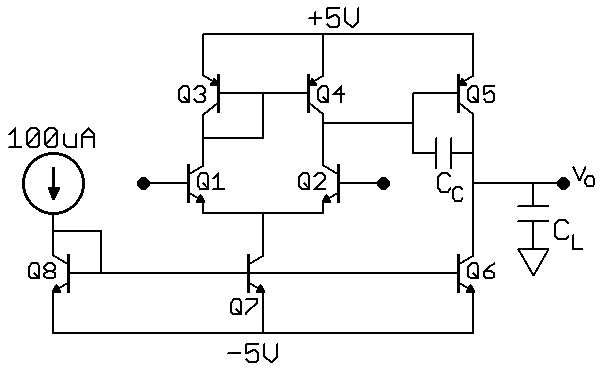
\includegraphics[width=0.75\textwidth]{npn-op.png}
\end{center}

\end{enumerate}
\clearpage
\subsection*{Problem 2: PNP Operational Amplifier}
Repeat problem 1 for the following PNP input OpAmp.  Create a summary table comparing both OpAmps.

\begin{center}
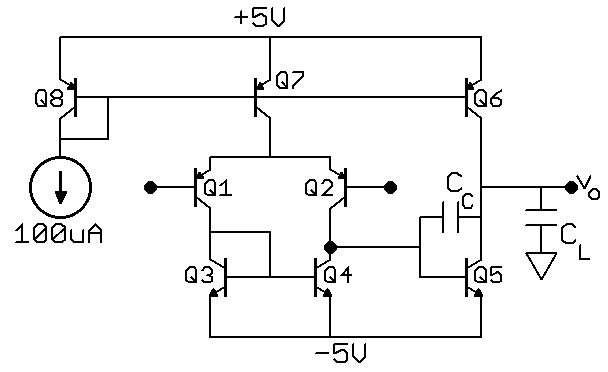
\includegraphics[width=0.75\textwidth]{pnp-op.png}
\end{center}

\subsection*{Problem 3: Variable Gain Compensator}
The LM101 was an excellent tool for the analog engineer in 1967.
It combined all of the advantages of integrated circuit technology with the flexibility of designing custom compensation networks for specific applications.
However, soon after the 101's debut, the LM741 (with an internal compensation capacitor) stole the show, and never again has an externally compensated opamp been on the market.

Modern fab processes far surpass the ones used to create the LM101, so even a perfectly designed compensation network on a 101 pales in comparison to the performance of a modern fixed compensation capacitor opamp.
One problem with making a modern externally compensated opamp is associated with the parasitic inductances and capacitances due to bond wires and packaging.
Bringing the feedback signal off-chip is simply not feasible.
To counter this, we can build a controllable compensation network on-chip.\\

For the following opamp:
\begin{enumerate}
	\item[(a)] Draw an approximate small signal model in terms of transistor parameters
	\item[(b)] Draw a block diagram based on the small-signal model
	\item[(c)] Find the closed-loop transfer function of the opamp
	\item[(d)] On one set of axes, draw the bode plot for A=[1,10,100]
\end{enumerate}

\begin{center}
Assume the following transistor parameters: \\
\begin{tabular}{| l | c | c |}
\hline
 & NPN & PNP \\
\hline
\hline
$\beta$	& 200 & 40 \\
\hline
$V_A$	& 50V & 20V \\
\hline
$\tau_F$ & 2.5ns & 25ns \\
\hline
$r_b,r_c$ & 0 & 0 \\
\hline
$c_\mu, c_{je}, c_{cs}$ & 0 & 0 \\
\hline
\hline
$C_c$ & 10pF & \\
\hline
\end{tabular}
\end{center}

\begin{center}
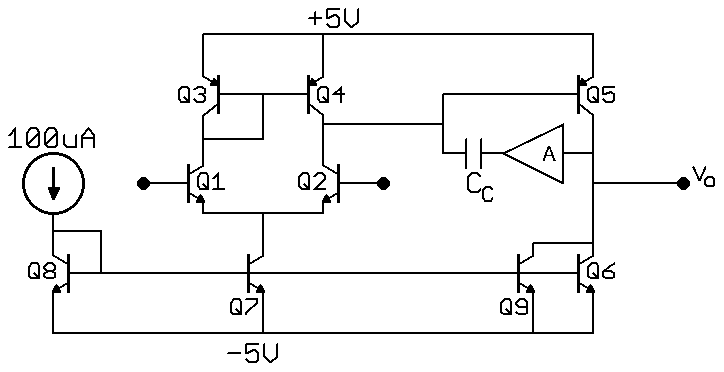
\includegraphics[width=0.75\textwidth]{comp-op.png}
\end{center}

\subsection*{Extra Credit}
Problem 3 implies that if we can control the compensator amplifier's gain, then we can tune the opamp's response to our liking.  Design a voltage controlled variable gain amplifier using transistor techniques we've discussed in class.
\end{document}
